% Preamble
\documentclass[11pt]{report}

% Packages
\usepackage{amsmath}
\usepackage{tikz}
%\usepackage{amstex}
\usetikzlibrary{calc}
\usetikzlibrary{decorations.markings}
\usetikzlibrary{decorations.pathmorphing,patterns}
\usepackage{transparent}
\usepackage{graphicx}
\usepackage{float}



\tikzstyle directed=[postaction={decorate,decoration={markings, % arrows on the field lines
mark=at position .1 with {\arrowreversed[scale=1.5]{stealth}},
mark=at position .9 with {\arrowreversed[scale=1.5]{stealth}}}}]
\tikzstyle tangent=[postaction={decorate,decoration={markings, % Tangent to the field line
mark=at position .7 with {\draw[ultra thick,stealth-,green!60!black,solid](-12pt,0)--(12pt,0)node[above]{$\vec{B}$};}}}]
\tikzstyle fLines=[thick,dashed,directed,tangent]

\title{Matura Project}
\author{Jan Wilhelm}
\date\today

\newcommand{\mycancel}[2]{\overset{#1}{\cancel{#2}}}
\renewcommand{\deg}[0]{\ensuremath{^\circ}}
\newcommand{\abs}[1]{\left|#1\right|}

\textheight=21cm
\oddsidemargin=-1.5cm
\textwidth=18.5cm
%\voffset=-5.5cm

% Document
\begin{document}
    \maketitle

    \tableofcontents
    \newpage


    \chapter{Introduction}\label{ch:introduction}
    \section{Abstract}\label{sec:abstract}
The question of whether a machine can beat a human in a specific task is as old as the first machines.
Machines have already surpassed humans in many areas, such as calculators, chess, and even driving cars (even though the laws do not allow it yet).
But what about foosball?
This project demonstrates the development of a machine-controlled goalkeeper for foosball, capable of reliably stopping slow balls.
While the goalkeeper occasionally struggles with the timing required for fast balls and shooting, the results serve as a proof of concept.
The machine uses a camera to monitor the game from below and motors to move the goalkeeper.
Although only basic AI was employed, the approach shows promise for extending similar designs to other players on the table.
This work highlights the potential of automated systems in fast-paced, real-time scenarios, while acknowledging room for improvement to enhance performance and timing.

\section{Introduction}\label{sec:introduction}
Whether a machine can surpass a human in a specific task has fascinated people since the first machines were created.
Over time, machines have outperformed humans in many areas, from simple calculations to complex strategy games like chess.
With advancements in AI, machines are now capable of tasks like driving cars, though they’re not widely used yet due to legal restrictions.

But can a machine beat a human in a game of foosball (table soccer)?
Unlike chess, foosball is fast-paced and unpredictable, requiring quick reflexes and real-time decision-making.
This makes it a perfect challenge for testing the limits of AI and robotics.

The goal of this project is to build a foosball-playing machine that can outperform a human.
The machine will rely on a camera to monitor the game from below and will be controlled by a computer using two motors per axis to move the players and shoot the ball.
The computer will use a neural network to determine the best moves—an interesting parallel, since the human brain is essentially a large neural network with billions of neurons.
%This project will explore how AI can handle complex, dynamic tasks like foosball and what this means for the future of AI .
The goal of this project is to build and test a foosball robot that can beat a human player.

\section{Motivation}\label{sec:motivation}
I love the combination of hardware and software—building a machine and then writing intelligent software to control it.
I also love playing foosball, so I thought it would be a great idea to combine these two interests.
The hardware itself will be challenging, but the software will be even more demanding, as it requires inventing new strategies that demand inhuman precision and speed.
The dream of playing foosball with precise, controlled moves would unlock a whole new level of strategy and fun.
Additionally, the machine could be used to teach and train people to play foosball, providing an innovative way to learn the game.
It would also enable a solo mode where a player could play against the machine at different difficulty levels, which would be an excellent way to practice and improve skills.


    \chapter{Calculations}\label{ch:calculations}
    \section{Objective}\label{sec:objective}

The primary objective of this project is to build a machine that can effectively compete with a human in foosball.
More specifically, the machine should be able to:

\begin{itemize}
    \item Defend against balls traveling at speeds of up to $7m/s$.
    This is approximately the speed achieved by normal players when they try to shoot fast.
    \item Shoot the ball back with a speed of $7m/s$.
    \item Achieve a positional precision of $0.1mm$, which is circa the accuracy of normal stepper motors (including the mechanics to move the players).
\end{itemize}


\section{Motors}\label{sec:motors}

\subsection{Objectives}\label{subsec:objectives}
I want to be able to defend a ball with a velocity of maximum $v=7m/s$.

\subsection{Table measurements}\label{subsec:table_measurements}
This picture shows the table with the measurements:

\begin{center}

    \begin{tikzpicture}
        \node[anchor=south west,inner sep=0] (image) at (0,0) {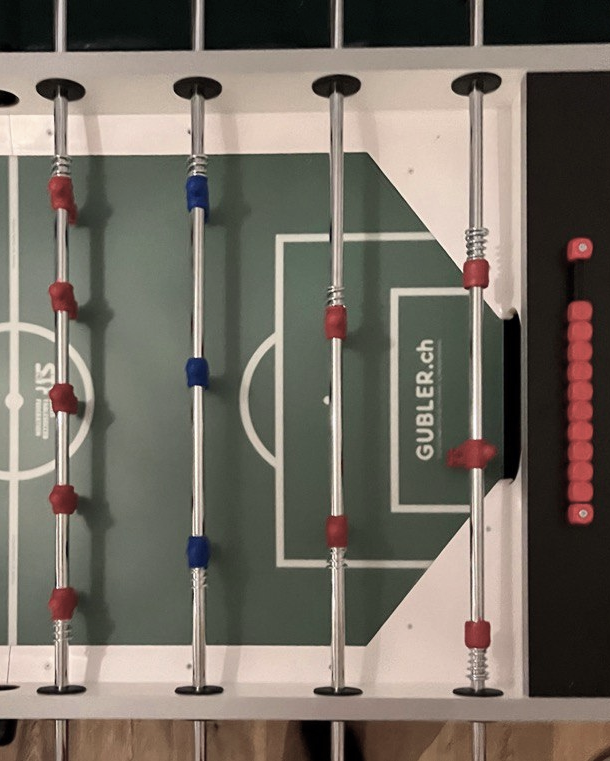
\includegraphics[width=0.5\textwidth]{../photos/foosball_table}};
        \begin{scope}
            [x={(image.south east)},y={(image.north west)}]
%        \draw[help lines,xstep=.1,ystep=.1] (0,0) grid (1,1);
%        \foreach \x in {0,1,...,9} { \node [anchor=north] at (\x/10,0) {0.\x}; }
%        \foreach \y in {0,1,...,9} { \node [anchor=east] at (0,\y/10) {0.\y}; }
            \def \tubex {0.76};
%        \draw[red,ultra thick,rounded corners] (0.62,0.65) rectangle (0.78,0.75);
            \draw[<->,blue!80!black!50,rounded corners, line width=1.5mm] (\tubex, 0.9)  -- (\tubex, 0.65) node[midway, left, fill=white, fill opacity=0.8,text opacity=1,rounded corners=2pt,inner sep=1pt] {\huge \textbf{180mm}};
            \draw[<->,blue!80!black!100,rounded corners, line width=1.5mm] (0.85, 0.9)  -- (0.85, 0.09) node[pos=0.85, left, fill=white, fill opacity=0.8,text opacity=1,rounded corners=2pt,inner sep=1pt] {\huge \textbf{700mm}};
            \draw[<->,blue!80!black!70,rounded corners, line width=1.5mm] (0.335, 0.5)  -- (0.775, 0.5) node[pos=0.85, left, fill=white, fill opacity=0.8,text opacity=1,rounded corners=2pt,inner sep=1pt] {\huge \textbf{400mm}};

        \end{scope}
    \end{tikzpicture}
\end{center}
%\todo{The calculations dont make completly sense, i think i made a mistake somewhere and bought an overpowered motor, which is fine i guess}

\subsection{Calculations for the moving motor}\label{subsec:moving_motor}
The distance from the foremost attacker to the goal is $s=0.4m$.
That means the player has to stop the ball in time t, where
\begin{equation}
    \label{eq:stopping_time}
    t = \frac{s}{v} = \frac{0.4m}{7m/s} = 0.057\dots s.
\end{equation}
Which is not a lot of time to process the image and move the motors.
I round the travel distance of the goalkeeper of 180mm to 200mm for the calculations, because there is a spring at the end of the either ends which can be compressed.
I always keep the goalkeeper in the middle, so the player has to travel a maximum distance of 0.1m that means the player has an average velocity of
\begin{equation}
    \label{eq:average_velocity}
    v = \frac{s}{t} = \frac{0.1m}{0.057s} = 1.75m/s.
\end{equation}
I assume a linear acceleration and deceleration, and when the player reaches the top speed it needs to decelerate immediately, so the acceleration and deceleration and therefore the force is as small as possible.
A graph to explain the velocity can be seen here:

\begin{center}
    \begin{tikzpicture}
        \centering
        \begin{axis}
            [
            axis x line=center,
            axis y line=center,
            width={0.2\linewidth},
            xtick=none,
            ytick={0,1},
            yticklabels={,$v_{max}$},
            xlabel={$t$},
            ylabel={$v$},
            xlabel style={below right},
            ylabel style={above left},
            xmin=-0.2,
            xmax=2.2,
            ymin=-0.2,
            ymax=1.2]

            \addplot [] table {
                0 0
                1 1
                2 0
            };
        \end{axis}
    \end{tikzpicture}
\end{center}

\noindent Which means the player has a top speed of at least $2\cdot1.75m/s=3.5m/s$, as the motors have to accelerate and decelerate.
The motor also needs to be able to accelerate the player in $0.057s/2=0.0285$, which means the motor needs to be able to achieve a maximum acceleration $a$ of
\begin{equation}
    \label{eq:acceleration}
    a = \frac{v}{t} = \frac{3.5m/s}{0.0285s} = 122.8m/s^2.
\end{equation}
I assume that the weight of the tubes is $m \approx 0.1kg$.
The torque needed to move the tubes is
\begin{equation}
    \label{eq:torque}
    \tau = F \cdot r = m \cdot a \cdot r = 0.1kg \cdot 122.8m/s^2 \cdot 0.083m \approx 1Nm
\end{equation}
assuming the radius $r_g$ of the gear is 8.3cm.
And the required top rotational speed (measured in rotations per minute $\text{RPM}$) is
\begin{equation}
    \label{eq:top_rpm}
    \frac{v}{2\pi r_g} \cdot 60s/min = \frac{7m/s}{2\pi \cdot 0.083m} \cdot 60s/min \approx 800\text{RPM}.
\end{equation}
A Motor that fits those requirements is the \textbf{PD42-3-1141\autocite{PD42-3-1141}} from \textbf{Trinamic}.

\subsection{Calculations for the rotating motor}\label{subsec:rotating_motor}
The ball has a mass $m=17g$.
I assume that I have an angle of $45\deg$ ($=\frac{\pi}{4}$ in radians) to accelerate the ball.
\\
\begin{center}

    \tikzset{
        testpic/.pic={
            \node at (0.05,-0.35) {
\includegraphics[height=3.2cm] {../photos/foosball_player}};
        },
        testpic2/.pic={
            \node at (0.05,-0.35) {
\includegraphics[height=3.2cm] {../photos/foosball_player}};
        },
    }

    \begin{tikzpicture}
        \def \r {2cm}
        \def \rsmall {0.5}
        \def \angle {45}
        \pic[rotate=45/2,transform shape] at (0,0) {testpic};
        \pic[rotate=-45/2,transform shape] at (0,0) {testpic2};
        \draw (0,0) -- ({-sin(\angle / 2)*\r}, {-cos(\angle / 2)*\r});
        \draw (0,0) -- ({sin(\angle / 2)*\r}, {-cos(\angle / 2)*\r}) node[right, midway] {$r_p=70\text{mm}$};
        \draw ({-sin(\angle / 2)*\rsmall}, {-cos(\angle / 2)*\rsmall}) arc(270-\angle/2:270+\angle/2:\rsmall) node[midway,below] {$45\deg$};
        \draw[->] ({-sin(\angle / 2)*\r}, {-cos(\angle / 2)*\r}) arc(270-\angle/2:270+\angle/2:\r) node[midway,below] {$l$};
%        \draw () circle (\r);
    \end{tikzpicture}
\end{center}
%    \\
That means the player has the distance $l$ to accelerate the ball together with the player.
\begin{equation}
    \label{eq:distance}
    l = r_p \cdot \frac{\pi}{4} = 70mm \cdot \frac{\pi}{4} = 55mm
\end{equation}
The goal is to shoot the ball back at a speed of 7m/s.
The time to accelerate the ball is
\begin{equation}
    \label{eq:time}
    t = \frac{2\pi\cdot r_p}{v} = \frac{2\pi\cdot 70mm}{7m/s} = \frac{\pi}{50} \approx 0.06s
\end{equation}
The maximum speed can easily be calculated with
\begin{equation}
    \label{eq:max_speed}
    \omega = \frac{60s/min}{t} = \frac{60s/min}{0.6s/rotation} = 1000\text{RPM}
\end{equation}
\todo{Compute the torque needed to accelerate the ball}
For the motor that just rotates the figure I can use a DC motor with gears and an encoder, as they often have more power and can go faster with less torque and accuracy.
% Pololu 10:1 Metal Gearmotor 37Dx65L mm 12V with 64 CPR Encoder (Helical Pinion) 4758
A motor that fits those requirements is the \textbf{Pololu 10:1 Metal Gearmotor 37Dx65L mm 12V with 64 CPR Encoder (Helical Pinion) 4758}\autocite{pololu-dc}.


\section{Camera}\label{sec:camera}

\subsection{Optics}\label{subsec:lens}
To achieve my goal of defending against balls at speed of up to $7m/s$, I need a camera that can capture the entire table at a framerate of at least 200fps.
I record the table from the bottom to avoid the players and the rods; therefore, I have to replace the floor of the table with a glass plate.
A sensor that achieves this is the \textbf{IMX287 CMOS} sensor from \textbf{Sony}.
This sensor has a width of $4.98\text{mm}$.
Here is a schematic of the approximate setup for the camera:\\
\begin{center}
    \begin{tikzpicture}
        \draw (0,0) -- (0, 5);
        \draw (0, 5) -- (10, 5);
        \draw (10, 5) -- (10, 0);

        \draw (1,0) -- (1, 4);
        \draw[red] (1, 4) -- (9, 4) node[pos=0.8, below] {Glass plate};
        \draw (9, 4) -- (9, 0);

        \draw (4.5, 0) -- (5.5, 0) node[below] {Sensor (4.98mm)};

        \pgfmathsetmacro{\lensRadius}{1}
        \pgfmathsetmacro{\lensHeight}{0.5}
        \pgfmathsetmacro{\startAngle}{asin(\lensHeight/\lensRadius)}

        \draw [fill=blue!15]  (4.5,\lensHeight)
        arc[start angle=180-\startAngle+90,delta angle=2*\startAngle,radius=\lensRadius]
        arc[start angle=-\startAngle+90,delta angle=2*\startAngle,radius=\lensRadius]
        -- cycle; % to get a better line end

        \draw[blue] (1, 4) -- (4.5, \lensHeight);
        \draw[blue] (4.5, \lensHeight) -- (5.5, 0);

        \draw[blue] (9, 4) -- (5.5, \lensHeight);
        \draw[blue] (5.5, \lensHeight) -- (4.5, 0);

        \draw[green] (1, 4) -- (5.5, \lensHeight);
        \draw[green] (5.5, \lensHeight) -- (5.5, 0);

        \draw[green] (9, 4) -- (4.5, \lensHeight);
        \draw[green] (4.5, \lensHeight) -- (4.5, 0);

        \draw (6.5, 0.5) node[]{Lens};
        \draw[<->] (5, 0.70) -- (5, 4) node[midway, right] {d};
        \draw[<->] (1, 4.2) -- (9, 4.2) node[above, midway] {FoV=Length of the foosball field};
    \end{tikzpicture}
\end{center}

\paragraph{Lens Equation}\label{par:lens_equation}

The relationship between the object width (FoV), sensor width, and distance to the object is given by:
\begin{equation}
    \text{Object Width (FoV)} = \text{Sensor Width} \times \frac{\text{Distance to Object (d)}}{\text{Focal Length (f)}}\label{eq:lens_equation}
\end{equation}


\noindent In my case $d = 700mm$ and my Field of View (FoV) is $1200mm$ as this is the length of the foosball field.
Now I solve for the focal length $f$:
\begin{equation}
    \label{eq:focal_length}
    f = \frac{\text{Sensor Width} \times \text{Distance to Object (d)}}{\text{Object Width (FoV)}} = \frac{4.98\text{mm} \times 700\text{mm}}{1200\text{mm}} \approx 2.9\text{mm}
\end{equation}
% Arducam 2.8-12mm Varifocal C-Mount Lens for Raspberry Pi HQ Camera, with C-CS Adapter
A lens that satisfies these requirements is the \textbf{Arducam 2.8-12mm Varifocal C-Mount Lens for Raspberry Pi HQ Camera, with C-CS Adapter} with a focal length of $2.8-12mm$.

    \chapter{Mechanics}\label{ch:mechanics}
    \section{Design}\label{sec:design}
The design has to be as simple as possible, because the more parts there are the more things can go wrong.
% maybe insert quote from elon musk lol
The main problem that one encounters when designing such a system is:
As soon as the motor moves the tube, and with it the player, the other motor cannot rotate the player anymore and vice versa.
To solve this problem, I have to design two parts/systems that can solve this problem.
%The first connects two tubes that can rotate freely but if one moves the other one moves with it.
%The second one is the opposite, it connects two tubes that can move freely back and forth but if one rotates the other one rotates with it.
Therefore, I have two main parts, I call them: Shoot Side and Move Side.

\subsection{Move Side}\label{subsec:move-side}
The Move Side is the part that moves the player back and forth.
I use a combination of a gear and a gear rack to move the player.
Additionally, I have a mechanism that connects the two tubes.
A render of the gears and the gear rack can be seen here:\\
%\begin{figure}[H]
%    \centering
%    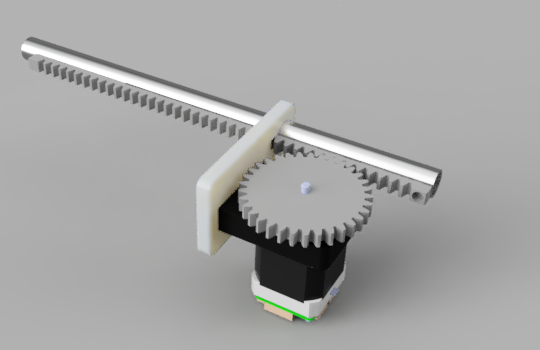
\includegraphics[height=7cm]{../photos/move_side_gear}
%    \caption[moveside1]{Move side gear and gear rack}
%    \label{fig:move_side_gear}
%\end{figure}

\noindent
\begin{tikzpicture}
    \node [anchor=west] (gear) at (-1,3.8) {\Large Gear};
    \node [anchor=west] (gear-rack) at (-1,6) {\Large Gear rack};
    \node [anchor=west, text width=2cm] (motor) at (-1,2) {\Large Motor \small \textbf{(PD42-3-1141)}};
    \node [anchor=east, text width=2cm] (holder) at (18,5) {\Large Holder \small connects the motor to the wall of the table};
    \node [anchor=east, text width=2cm] (tube) at (18,2) {\Large Tube};
    \begin{scope}[xshift=1.5cm]
        \node[anchor=south west,inner sep=0] (image) at (0,0) {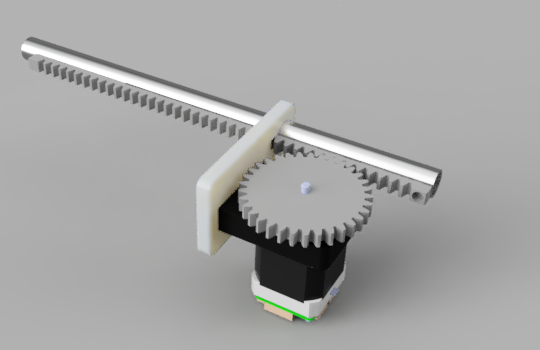
\includegraphics[width=0.7\textwidth]{../photos/move_side_gear}};
        \begin{scope}
            [x={(image.south east)},y={(image.north west)}]
%            \draw[red,ultra thick,rounded corners] (0.48,0.80) rectangle (0.55,0.95);
%            \draw [-latex, ultra thick, red] (note) to[out=0, in=-120] (0.48,0.80);
%            \draw [-stealth, line width=5pt, cyan] (water) -- ++(0.4,0.0);
            \draw [-stealth, line width=2pt, red] (gear) -- ++(0.65, 0.0);
            \draw [-stealth, line width=2pt, red] (motor) -- ++(0.60, 0.0);
            \draw [-stealth, line width=2pt, red] (gear-rack) -- ++(0.35, 0.0);
            \draw [-stealth, line width=2pt, red] (holder) -- ++(-0.74, 0.0);
            \draw [-latex, ultra thick, red] (tube) to[out=180, in=-25] ++(-0.39,0.23);
        \end{scope}
    \end{scope}
\end{tikzpicture}%

% Todo: insert a picture of the meachaism that connects the tubes
\todo{Insert real life image}

\subsection{Shoot Side}\label{subsec:turn-side}
The Shoot Side is the part that rotates the player.
The turning motor is connected to a tube containing the smaller tube on which the player sits.
The larger tube contains a slit along its length, and the smaller tube has a pin that fits (a screw in this case) into the slit.
A render of the turning mechanism can be seen here:

\noindent

\scalebox{0.9}{

\begin{center}
    \begin{tikzpicture}
%    [
%transform canvas={scale=1}
%]

%        \useasboundingbox (-6.0,-6.3) rectangle (6.0,9.5);
        \node [anchor=west, text width=2cm] (motor) at (-1,4.6) {\Large Motor \small \textbf{(Pololu)}};
        \node [anchor=east, text width=3cm] (larger-tube) at (18.5,9) {\Large Larger tube \small connected to the motor};
        \node [anchor=east, text width=3cm] (main-tube) at (18.5,6.95) {\Large Main tube \small connected to the player};
        \node [anchor=east, text width=3cm] (slit) at (18.5,5.5) {\Large Slit};
        \node [anchor=east, text width=3cm] (pin) at (18.5,3.5) {\Large Pin};
        \node [anchor=east, text width=3cm] (holder) at (18.5,1.5) {\Large Holder \small connects the motor to the wall of the table};
        \begin{scope}[xshift=1.5cm]
            \node[anchor=south west,inner sep=0] (image) at (0,0) {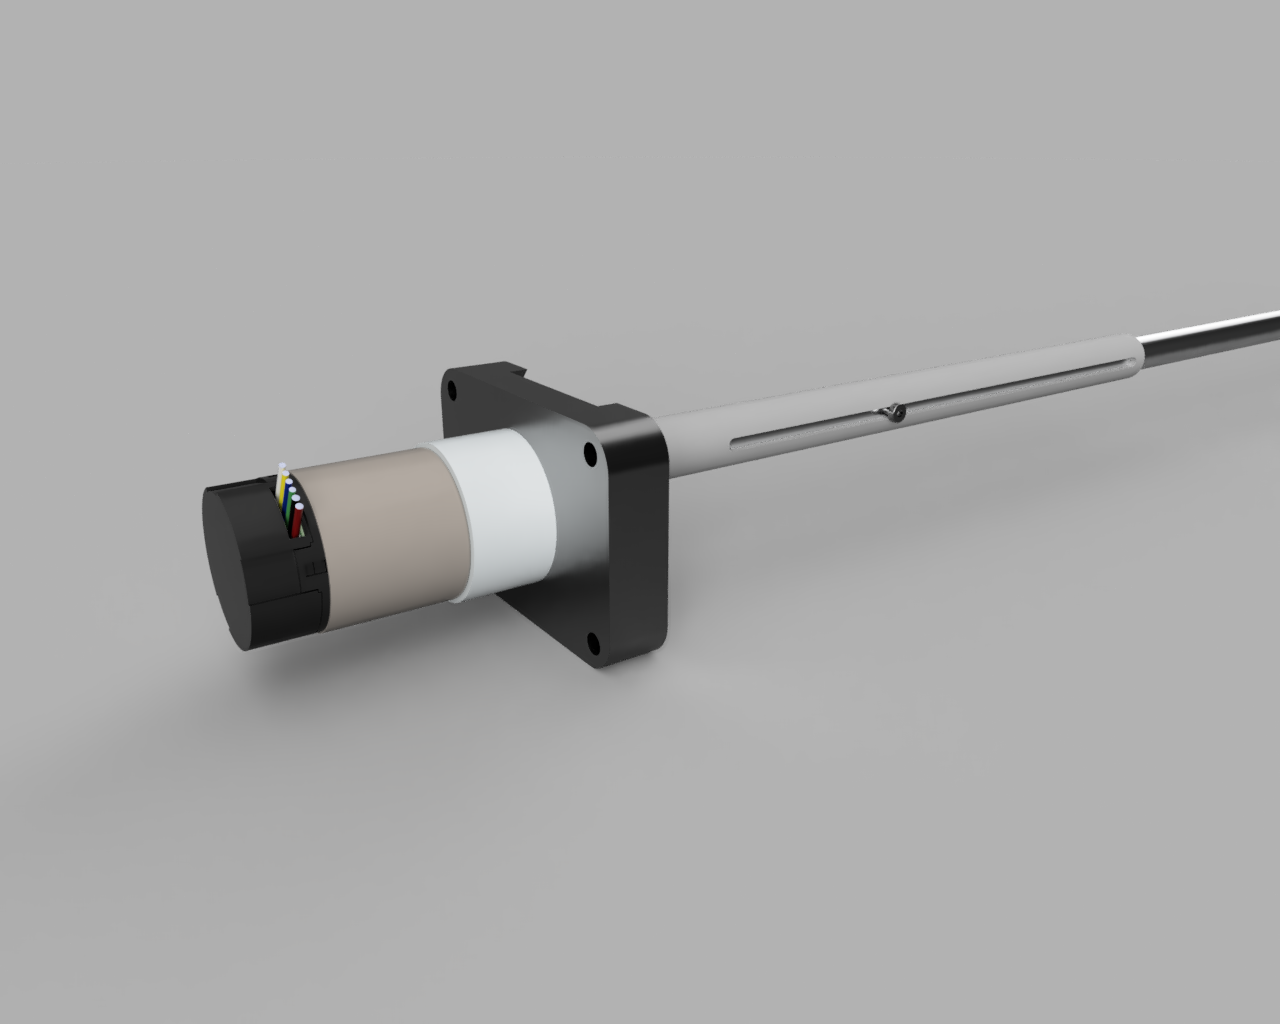
\includegraphics[width=0.7\textwidth]{../photos/turn_side}};
            \begin{scope}
                [x={(image.south east)},y={(image.north west)}]
%                \draw[blue, thick] (-0.2,0) rectangle (1.3,1);
                \useasboundingbox (-0.2,0) rectangle (1.3,1);
%            \draw[red,ultra thick,rounded corners] (0.48,0.80) rectangle (0.55,0.95);
%            \draw [-latex, ultra thick, red] (note) to[out=0, in=-120] (0.48,0.80);
%            \draw [-stealth, line width=5pt, cyan] (water) -- ++(0.4,0.0);
                \draw [-stealth, line width=2pt, red] (motor) -- ++(0.25, 0.0);
                \draw [-stealth, line width=2pt, red] (larger-tube) to[out=180, in=90] ++(-0.6, -0.29);
                \draw [-stealth, line width=2pt, red] (main-tube) -- ++(-0.21, 0.0);
                \draw [-stealth, line width=2pt, red] (slit) to[out=180, in=-90] ++(-0.4, 0.08);
                \draw [-stealth, line width=2pt, red] (pin) to[out=180, in=-90] ++(-0.515, 0.245);
                \draw [-stealth, line width=2pt, red] (holder) to[out=180, in=-60] ++(-0.715, 0.2);
%            \draw [-latex, ultra thick, red] (tube) to[out=180, in=-25] ++(-0.33,0.25);
            \end{scope}
        \end{scope}

    \end{tikzpicture}
\end{center}
}

%\todo{Insert real life image}



    \section{Frame}\label{sec:frame}


    \chapter{Electronics}\label{ch:electronics}


    \chapter{Software}\label{ch:software}
    \section{General}\label{sec:general}
The software has the task to gather the image information from the camera, detecting the ball, predicting where it will go in the future and controlling the motors to either stop or shoot the ball.
This task can be split into the following chapters:
\begin{itemize}
    \item \textbf{Optics}: Correcting for Lens distortion and converting the pixel coordinates to real world coordinates
    \item \textbf{Ball Detection}: Detecting the ball in the image
    \item \textbf{Prediction}: Predicting the ball movement
    \item \textbf{Controlling the motors}: Finally, we move the motors to the correct position
\end{itemize}


\section{Optics}\label{sec:optics}
The goal here is to correct for lens distortion, this can be achieved by first capturing many images containing a checkerboard pattern with known gird size, in this is case 8x8.
One such image in my case looks like this:
\begin{figure}[H]
    \centering
    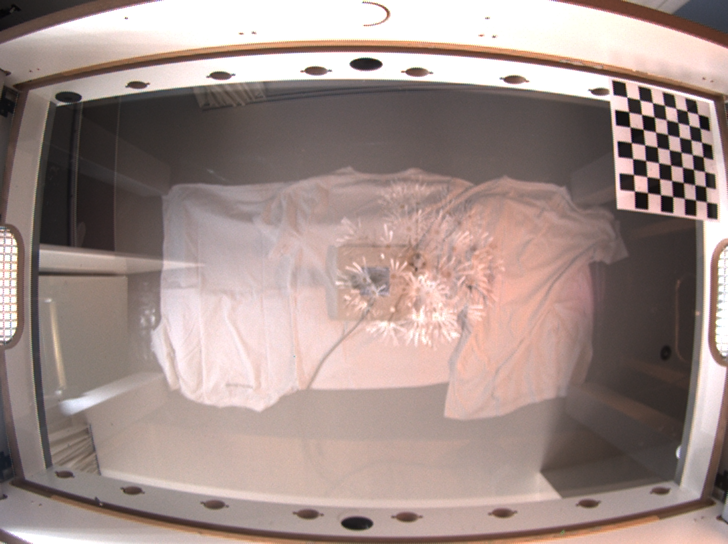
\includegraphics[height=5cm]{../photos/calibration_image}
    \caption[calimage]{Calibration image}
    \label{fig:calibration_image}
\end{figure}
As one can see there is severe distortion in the image, this can be corrected by using the OpenCV library.

% todo: should i explain in detail how opencv does it?
% lets do it and later i can delete it if its too much

\subsection{OpenCV}\label{subsec:opencv}
OpenCV is a library that provides many functions for image processing, one of these functions is the camera calibration function.
The function takes the images of the checkerboard pattern and calculates the distortion coefficients and the camera matrix.

The key principal is to map the distorted image to an undistorted image, this is done by calculating the pixel coordinates of the undistorted image for each pixel in the distorted image.
The Formulas for this are:
\begin{itemize}
    \item \textbf{Radial distortion:} This is the distortion that makes straight lines appear curved:
    \begin{gather*}
        r^2 = x^2 + y^2\\
        x_{\text{radial}} = x(1 + k_1 r^2 + k_2 r^4 + k_3 r^6)\\
        y_{\text{radial}} = y(1 + k_1 r^2 + k_2 r^4 + k_3 r^6)\\
    \end{gather*}
    \item \textbf{Tangential distortion:} This distortion occurs because the lens and the image sensor are not perfectly parallel.
    \begin{gather*}
        x_{\text{tangential}} = 2p_1 xy + p_2(r^2 + 2x^2)\\
        y_{\text{tangential}} = p_1(r^2 + 2y^2) + 2p_2 xy\\
    \end{gather*}
\end{itemize}
Together that gives:
\begin{gather*}
    x' = x_{\text{radial}} + x_{\text{tangential}}\\
    y' = y_{\text{radial}} + y_{\text{tangential}}\\
\end{gather*}
Finally, the undistorted pixel positions are transformed back to image coordinates using the camera matrix \( K \):
\[
    \begin{bmatrix}
        u \\
        v
    \end{bmatrix}
    =
    K \cdot
    \begin{bmatrix}
        x' \\
        y' \\
        1
    \end{bmatrix}
\]
where $K$ is the camera matrix:
\begin{center}
    K = \begin{bmatrix}
            f_x & 0   & c_x \\
            0   & f_y & c_y \\
            0   & 0   & 1
    \end{bmatrix}\\
    where:
\end{center}
\begin{itemize}
    \item $f_x$ and $f_y$ are the focal lengths along the x and y axes (in pixels),
    \item $c_x$ and $c_y$ are the coordinates of the optical center (principal point), typically at the center of the image.
\end{itemize}
These formulas allow the distorted image points to be remapped to undistorted coordinates.

\subsubsection{Implementation}\label{subsubsec:implementation}


Using the undistort function provided by opencv is not fast enough for our needs, because we only have 3ms to do the whole image processing and motor controlling.
So I wrote a custom function that generates a table where the index for each pixel in the new image is stored, so the function doesnt have to calculate the pixel coordinate for the undistorted image each time when the function is called.
The rust function to get the coordinates $x_{\text{original}},y_{\text{original}}$ of a pixel at $x_{\text{undistorted}},y_{\text{undistorted}}$ in the distorted (original) image looks like this:



\begin{lstlisting}[language=rust,breaklines,label={lst:distort_coords}]
/// Calculate the distorted coordinates given undistorted image coordinates.
fn distort_coords(x: f64, y: f64, fx: f64, fy: f64, cx: f64, cy: f64) -> (f64, f64) {
    // Distortion coefficients
    let k1 = DIST_COEFFS[0];
    let k2 = DIST_COEFFS[1];
    let p1 = DIST_COEFFS[2];
    let p2 = DIST_COEFFS[3];
    let k3 = DIST_COEFFS[4];

    // Normalize coordinates to [-1, 1]
    let x_normalized = (x - cx) / fx;
    let y_normalized = (y - cy) / fy;

    // Calculate radial distance
    let r2 = x_normalized * x_normalized + y_normalized * y_normalized;
    let r4 = r2 * r2;

    // Apply radial distortion
    let radial_distortion = 1.0 + k1 * r2 + k2 * r4 + k3 * r4 * r2;
    let x_radial = x_normalized * radial_distortion;
    let y_radial = y_normalized * radial_distortion;

    // Apply tangential distortion
    let x_tangential =
        2.0 * p1 * x_normalized * y_normalized + p2 * (r2 + 2.0 * x_normalized * x_normalized);
    let y_tangential =
        p1 * (r2 + 2.0 * y_normalized * y_normalized) + 2.0 * p2 * x_normalized * y_normalized;

    // Distorted coordinates
    let x_distorted = x_radial + x_tangential;
    let y_distorted = y_radial + y_tangential;

    // Map back to pixel coordinates
    let distorted_x = fx * x_distorted + cx;
    let distorted_y = fy * y_distorted + cy;

    (distorted_x, distorted_y)
}
\end{lstlisting}
Where \texttt{DIST\_COEFFS} are the distortion coefficients calculated by the OpenCV calibration function.
To generate the table I used the following code:
\begin{lstlisting}[language=rust,breaklines,label={lst:gen_table}]
/// Generate precomputation table for undistortion.
pub fn gen_table(
    original_width: u32, original_height: u32,
    new_width: u32, new_height: u32,
    x_offset: i32, y_offset: i32,
) -> Vec<i32> {
    // Camera matrix values
    let fx = CAMERA_MATRIX[0][0];
    let fy = CAMERA_MATRIX[1][1];
    let cx = CAMERA_MATRIX[0][2];
    let cy = CAMERA_MATRIX[1][2];
    let mut precomputation_table = vec![];

    for y in 0..new_height {
        for x in 0..new_width {
            let x = x as i32 + x_offset;
            let y = y as i32 + y_offset;
            // Map the pixel back to the distorted image coordinates
            let (distorted_x, distorted_y) = distort_coords(x as f64, y as f64, fx, fy, cx, cy);

            let distorted_x = distorted_x.round() as i32;
            let distorted_y = distorted_y.round() as i32;

            // If the coordinates are within the bounds of the original image, map the pixel
            let index = if distorted_x >= 0
                && distorted_x < original_width as i32
                && distorted_y >= 0
                && distorted_y < original_height as i32
            {
                let index = ((distorted_y * original_width as i32 + distorted_x) * 3) as usize;
                index as i32
            } else {
                -1 // black pixel (outside the image bounds)
            };
            precomputation_table.push(index);
        }
    }
    precomputation_table
}
\end{lstlisting}
This generates a long vector with the corresponding index for each pixel in the undistorted image.
(Note that these are indices because the image is flattened to a vector of length $3 \cdot \text{width} \cdot \text{height}$, where each pixel has 3 values for the RGB channels.)

Using the table is as simple as just looking up the index for the pixel in the undistorted image and copying the pixel values from the original image to the new image.
This function is called for each frame and the result is a corrected image with no distortion.
The Code can be seen here:
\begin{lstlisting}[language=rust,breaklines,label={lst:undistort_image_table}]
/// Undistort an image using the precomputed table.
pub fn undistort_image_table(
    img: &[u8],
    undistorted_img: &mut [u8],
    table: &Vec<i32>,
    new_width: u32,
    new_height: u32,
) {
    // Assert that the image has the correct size
    assert_eq!(
        undistorted_img.len(),
        3 * new_width as usize * new_height as usize
    );

    for i in 0..new_height * new_width {
        let index = table[i as usize];

        if index != -1 {
            #[inline]
            /// Helper function to avoid code duplication
            fn set_pixel(undistorted_img: &mut [u8], img: &[u8], pixel_index: usize, i: usize) {
                undistorted_img[i as usize] = img[pixel_index];
            }
            let pixel_index = index as usize;
            set_pixel(undistorted_img, img, pixel_index, i as usize * 3);
            set_pixel(undistorted_img, img, pixel_index + 1, i as usize * 3 + 1);
            set_pixel(undistorted_img, img, pixel_index + 2, i as usize * 3 + 2);
        }
    }
}
\end{lstlisting}
The parameters for this function are a bit special because one argument is the final vector where the undistorted image is stored, the other is the original image, and the last one is the table that was generated before.
Giving the final image buffer as a parameter saves time, because the image buffer can be reused in each frame, saving the time to reallocate the buffer each frame.
\\
An illustration can be seen in this example rainbow image being given to the undistort function:
% todo: pick a better example image
\begin{figure}[H]
    \centering
    \begin{subfigure}{.5\textwidth}
        \centering
        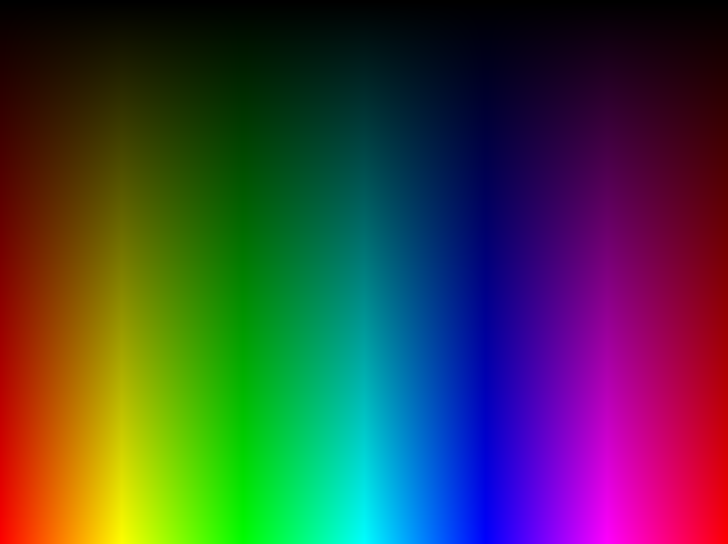
\includegraphics[width=.8\textwidth]{../photos/original_rainbow}
        \caption[originalRainbow]{Original rainbow image}
        \label{fig:original_rainbow}
    \end{subfigure}%
    \begin{subfigure}{.5\textwidth}
        \centering
        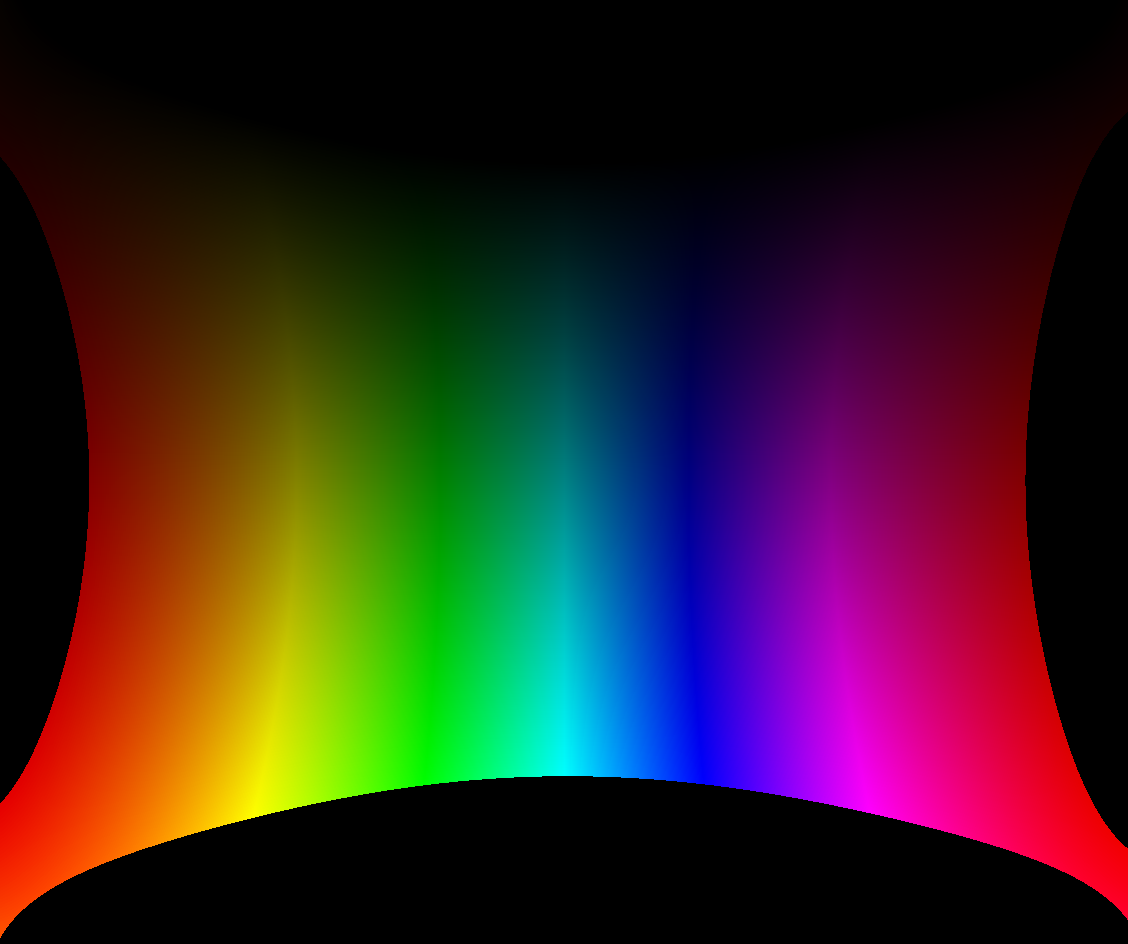
\includegraphics[width=.8\textwidth]{../photos/undistorted_rainbow}
        \caption[originalRainbow]{Undistorted rainbow image}
        \label{fig:undistorted_rainbow}
    \end{subfigure}
    \caption{Undistorted rainbow image}
    \label{fig:original_undistorted_rainbow}
\end{figure}
The undistorted image~\ref{fig:undistorted_rainbow} is larger than the original rainbow image~\ref{fig:original_rainbow}, that is because some pixel are moved out of the original image bounds because the camera can see "further" at the corners than at the sides.
This effect can also be seen in some example footage of the table:
\begin{figure}[H]
    \centering
    \begin{subfigure}{.5\textwidth}
        \centering
        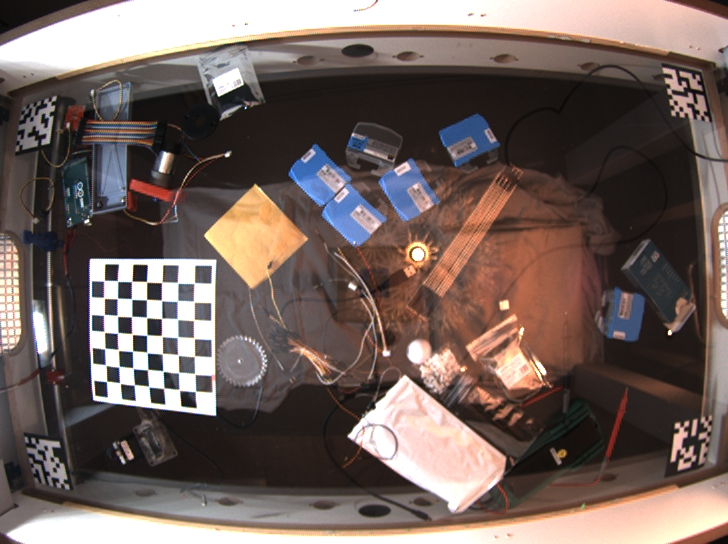
\includegraphics[width=.8\textwidth]{../photos/original_example8}
        \caption[originalRainbow]{Original image}
        \label{fig:original_example8}
    \end{subfigure}%
    \begin{subfigure}{.5\textwidth}
        \centering
        \includegraphics[width=.8\textwidth]{../photos/output8}
        \caption[originalRainbow]{Undistorted image}
        \label{fig:undistorted_example8}
    \end{subfigure}
    \caption{Undistorted example image}
    \label{fig:original_undistorted_example}
\end{figure}
Therefore we have to crop the image at the sides by a different amount, I made a simple graphical user interface (GUI) to adjust the cropping values.
The GUI can be seen here:
\begin{figure}[H]
    \centering
    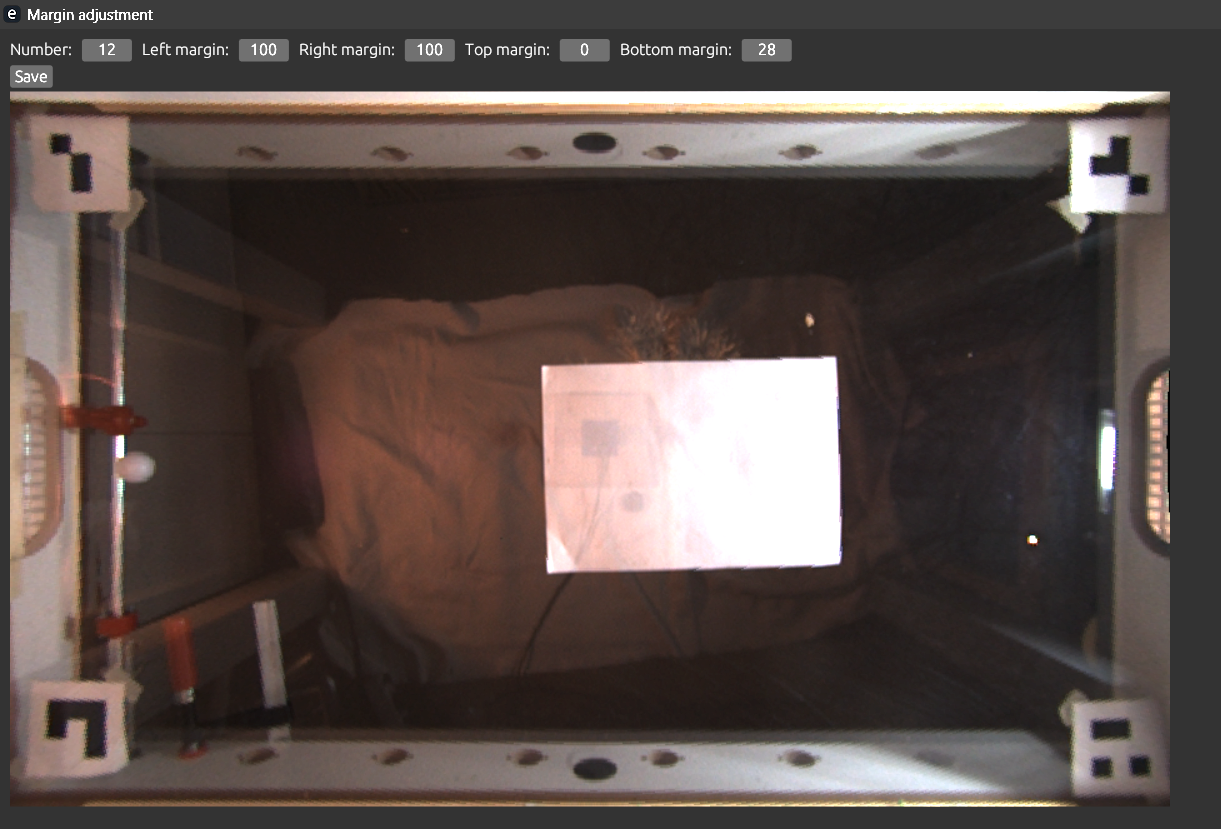
\includegraphics[width=0.8\textwidth]{../photos/margin_adj_gui}
    \caption[marginadjgui]{Margin Adjustment GUI}
    \label{fig:margin_adj_gui}
\end{figure}
The GUI is also written in rust using the egui\autocite{egui} library.
\todo{Fix the egui cite command (numbers instead of name)}
The cropped example image looks like this:
\begin{figure}[H]
    \centering
    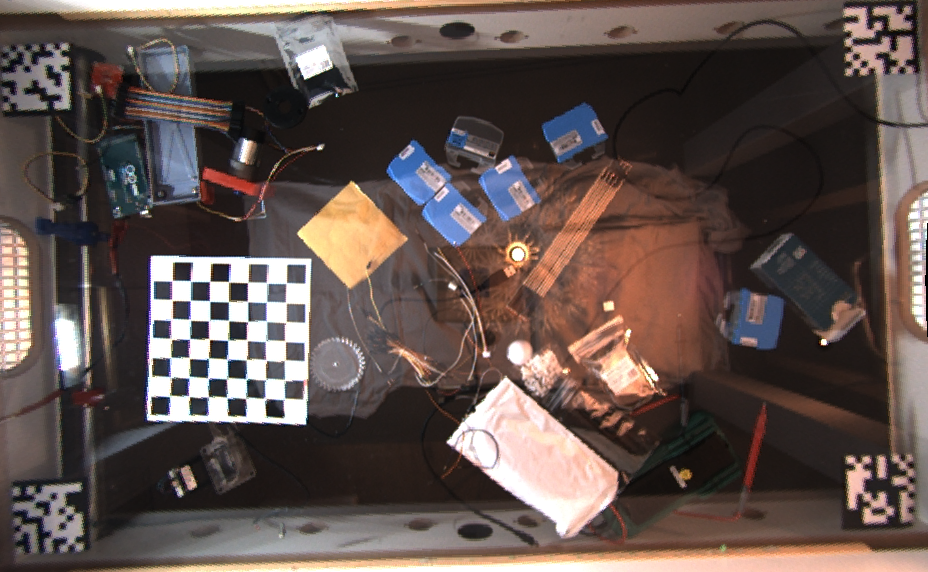
\includegraphics[width=0.8\textwidth]{../photos/example8_cropped}
    \caption[croppedexampleimage]{Cropped example image}
    \label{fig:example8_cropped}
\end{figure}

\subsection{Real World Coordinates}\label{subsec:real-world-coordinates}
An important part of the software is to convert the pixel coordinates to real-world coordinates.
This is done by adding fiducials (markers that are known to be at a specific position) to the table.
The fiducials are placed at the corners of the table, and the coordinates are measured in millimeters.
They can be seen here:
\begin{figure}[H]
    \centering
    \begin{subfigure}{.2\textwidth}
        \centering
        \fbox{
\includegraphics[width=.7\textwidth]{../photos/fiducials/fiducial_1}}
        \caption[originalRainbow]{Fiducial 1}
        \label{fig:fid_1}
    \end{subfigure}%
    \begin{subfigure}{.2\textwidth}
        \centering
        \fbox{
\includegraphics[width=.7\textwidth]{../photos/fiducials/fiducial_2}}
        \caption[originalRainbow]{Fiducial 2}
        \label{fig:fid_2}
    \end{subfigure}
    \begin{subfigure}{.2\textwidth}
        \centering
        \fbox{
\includegraphics[width=.7\textwidth]{../photos/fiducials/fiducial_3}}
        \caption[originalRainbow]{Fiducial 3}
        \label{fig:fid_3}
    \end{subfigure}
    \begin{subfigure}{.2\textwidth}
        \centering
        \fbox{
\includegraphics[width=.7\textwidth]{../photos/fiducials/fiducial_4}}
        \caption[originalRainbow]{Fiducial 4}
        \label{fig:fid_4}
    \end{subfigure}
    \caption{Fiducials}
    \label{fig:fiducials_all}
\end{figure}
To calibrate the real world coordinates one has to detect the fiducials reliably in the image.
This can be done by using a convolutional neural network (CNN) to detect the fiducials.

\subsubsection{Training Data}\label{subsubsec:training-data}
To train the CNN, one needs a lot of images containing the fiducials, making such a lot of images and then checking where exactly the coordinates of the midpoint of the fiducial lies is very tedious and not practical.
Therefore i wrote a Java programm to generate about 250 labeled images to train the CNN.
An image containing all the fiducials looks like this (the red point shows the midpoint of the fiducial):
\begin{figure}[H]
    \centering
    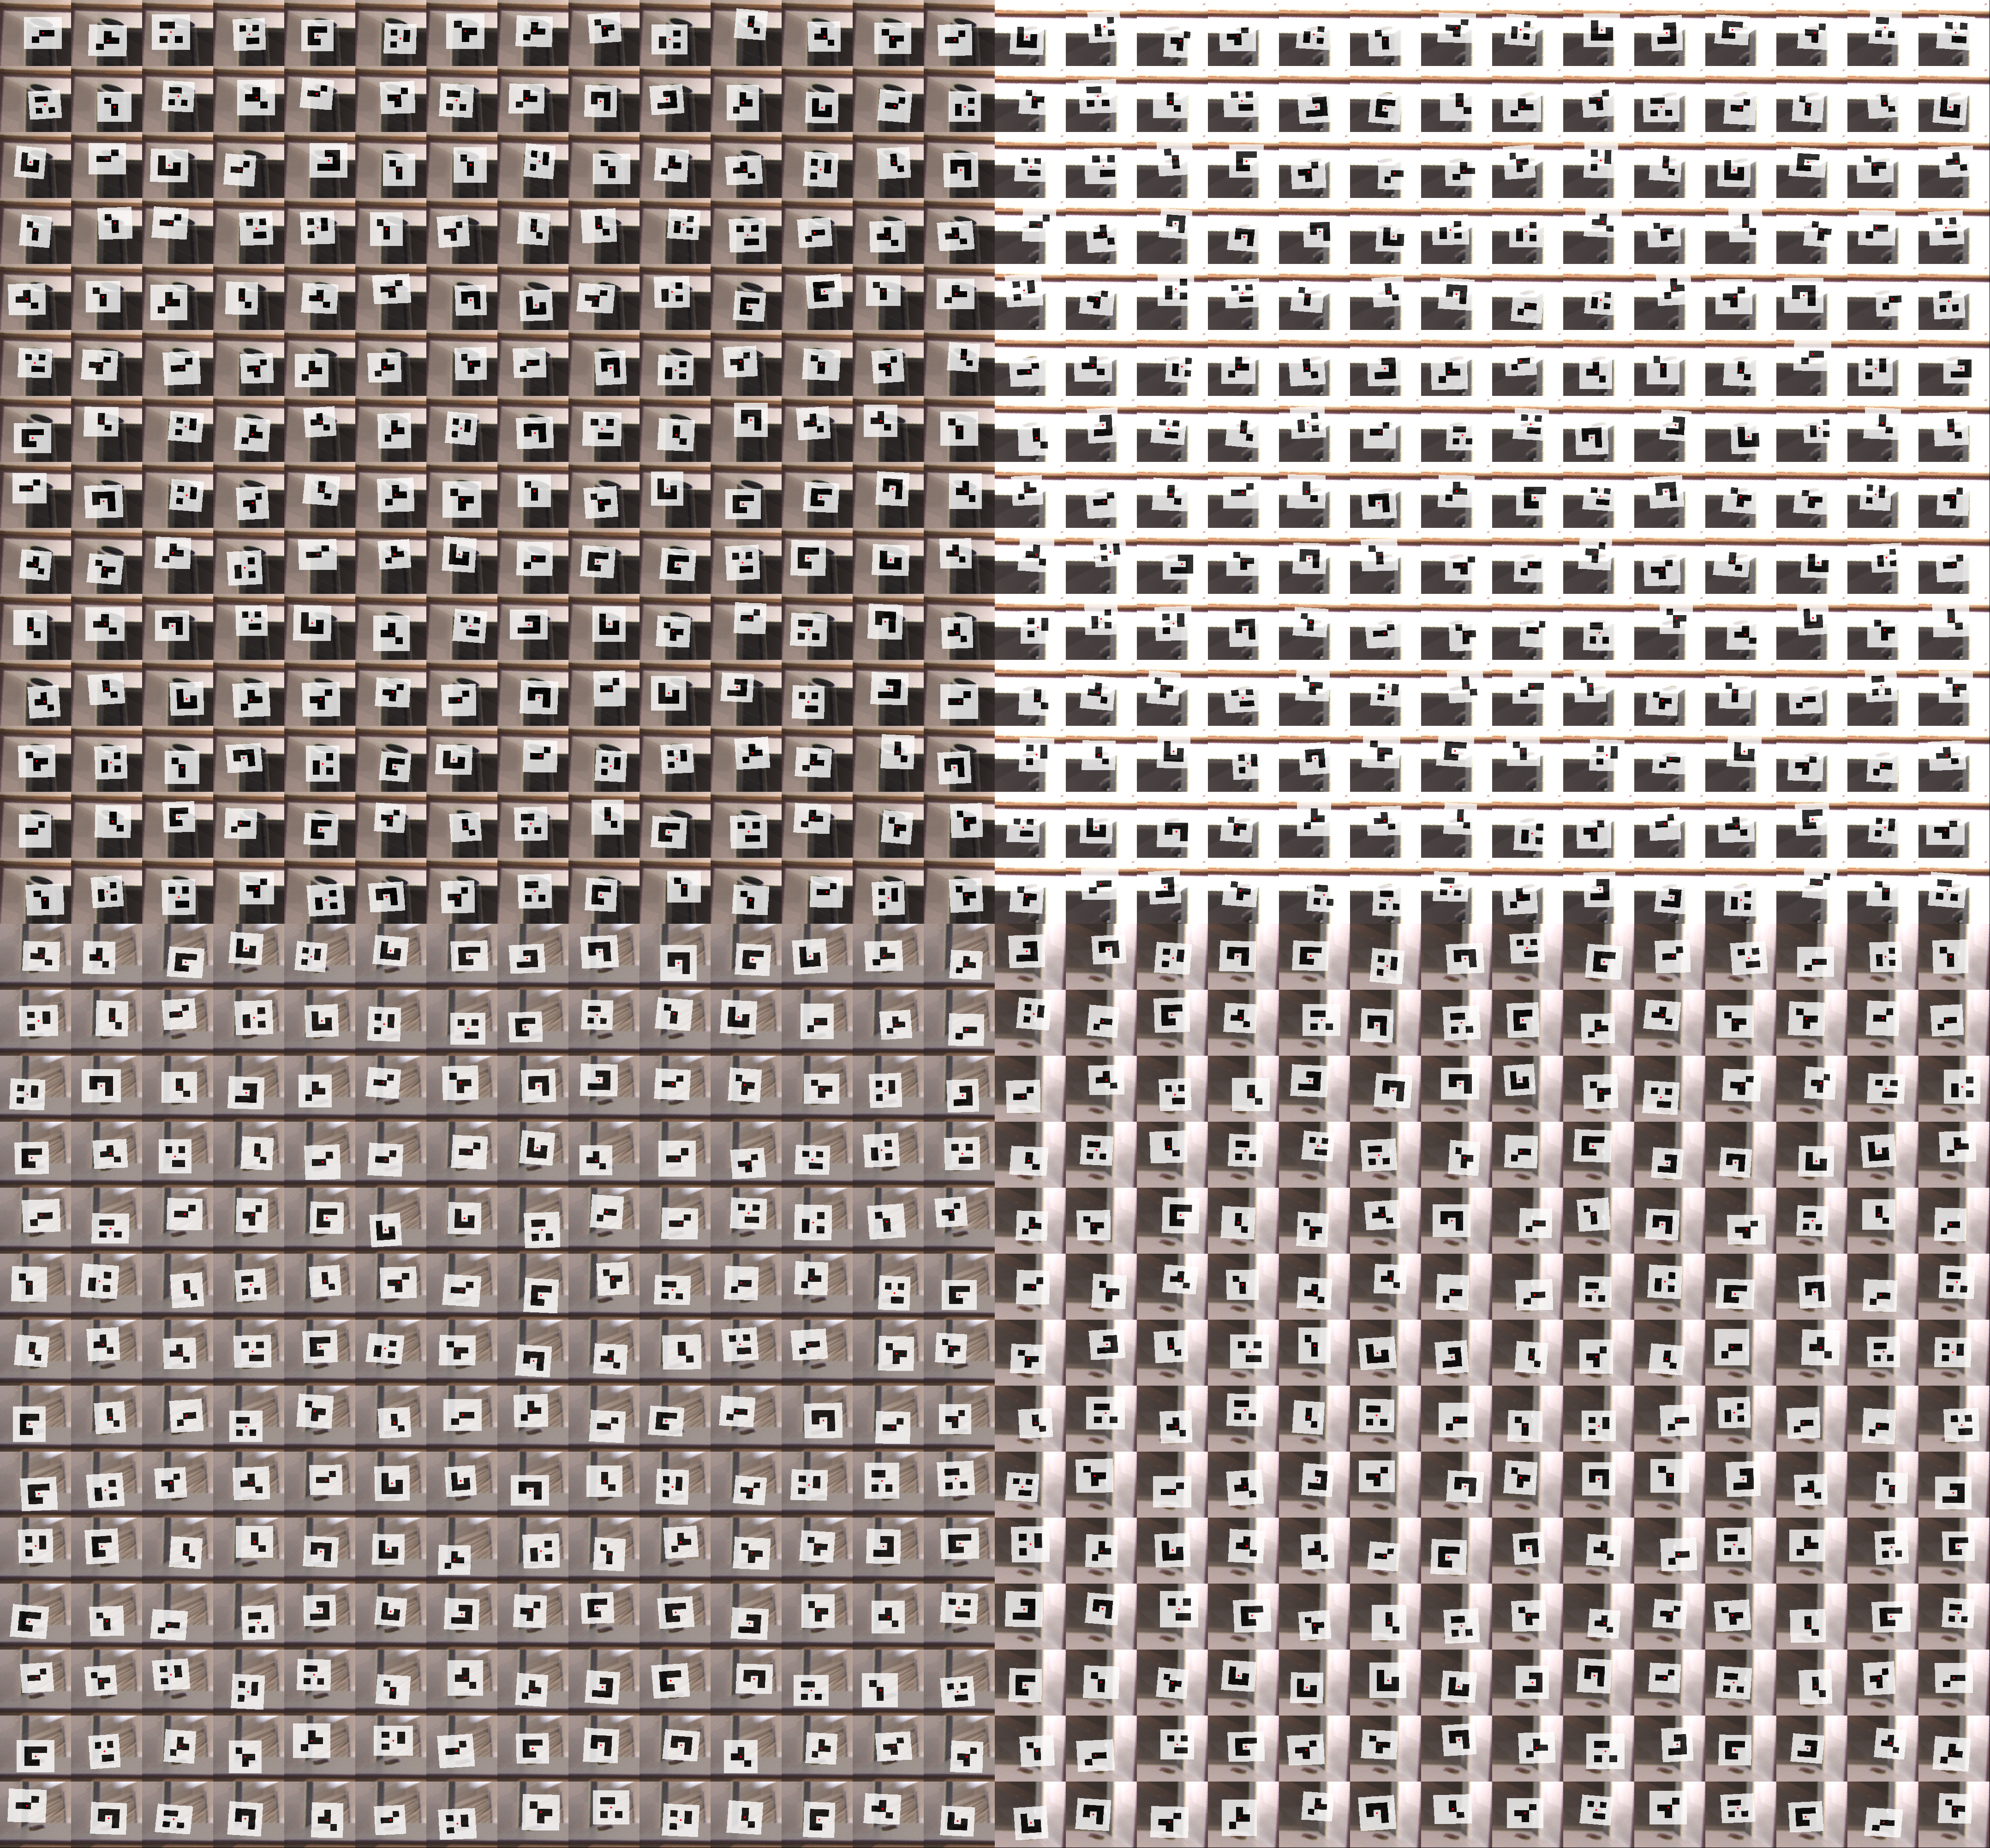
\includegraphics[width=0.8\textwidth]{../photos/training_whole_general_image}
    \caption[fiducials]{Training fiducials}
    \label{fig:fiducials}
\end{figure}
The trick I am using is that I know that the fiducials always lie in the corners of the table, so I can generate the images by just placing the fiducials in the corners with some random offset.
The different parts can be seen here:

\begin{figure}[H]
    \centering
    \begin{tikzpicture}
        % Include the image
        \node[anchor=south west, inner sep=0] (image) at (0,0) {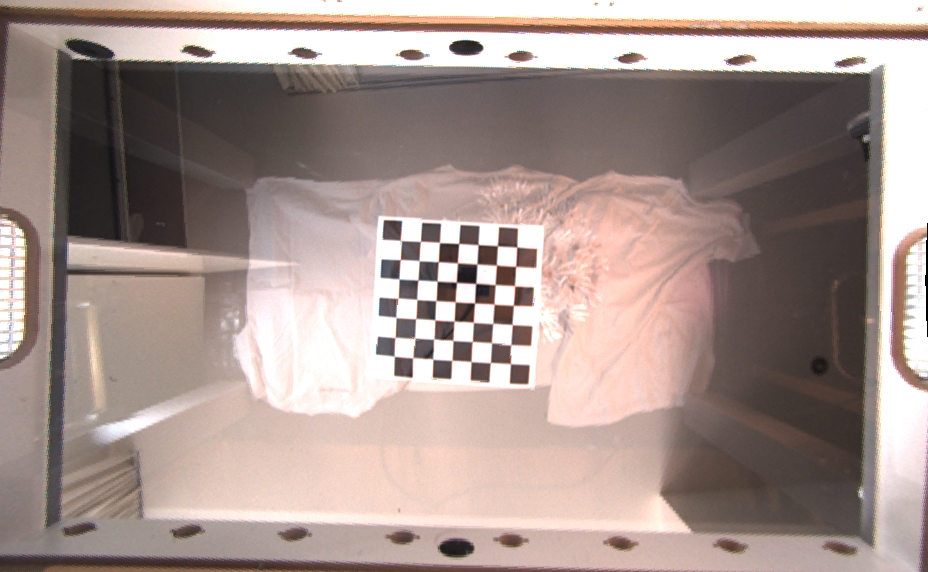
\includegraphics[width=0.8\textwidth]{../photos/base_img}};
        \begin{scope}
            [x={(image.south east)}, y={(image.north west)}]
            % vertical lines (6 parts)
            \foreach \i in {1/6, 2/6, 3/6, 4/6, 5/6} {
                \draw[red, very thick] (\i, 0) -- (\i, 1);
            }
            % horizontall lines (4 parts)
            \foreach \i in {1/4, 2/4, 3/4} {
                \draw[red, very thick] (0, \i) -- (1, \i);
            }
        \end{scope}
    \end{tikzpicture}
    \caption{Image split into 4 horizontal and 6 vertical parts}\label{fig:figure}
\end{figure}
\textbf{Create and Train the CNN}\\
I made two separate CNNs, one for detecting the fiducial (number from 1-4 as there are four fiducials) (also known as classification) and one for detecting the coordinate of the midpoint of the fiducial (from where the real-world measurements are made).
The CNNs are trained using the tensorflow library made by google.
The structure of the CNNs can be seen here:
\begin{figure}[H]
    \centering
    \begin{subfigure}{.5\textwidth}
        \centering
        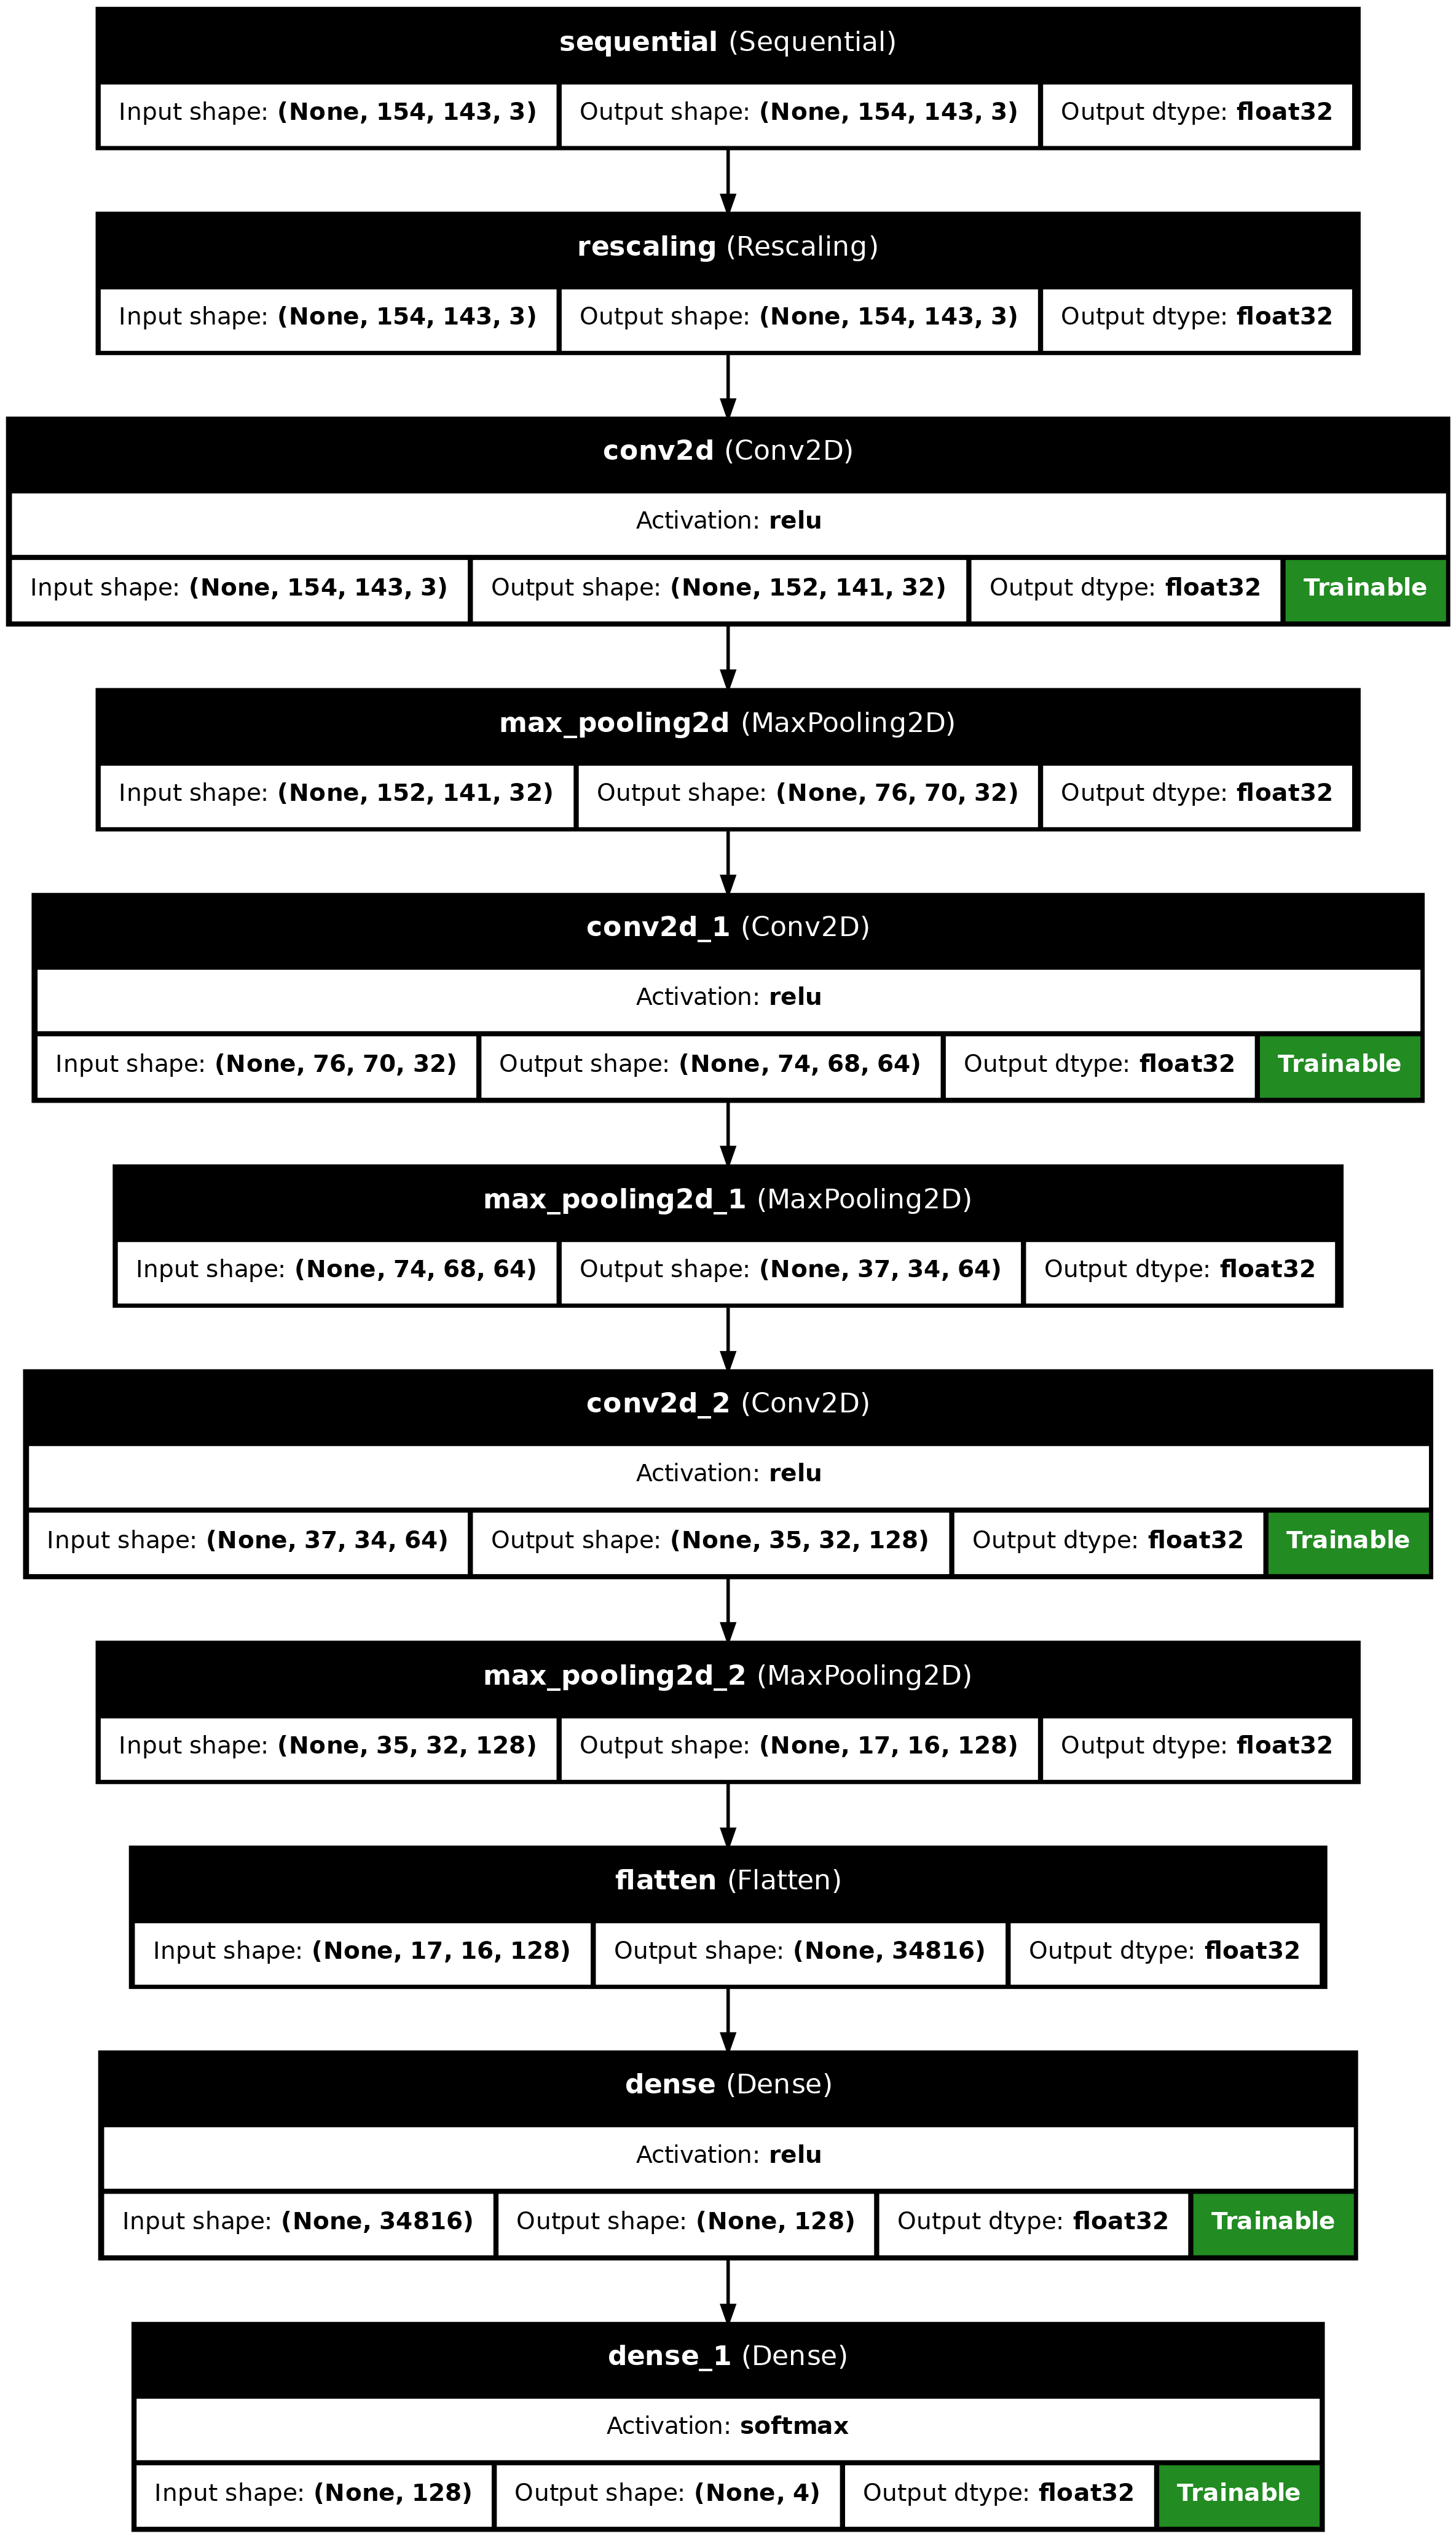
\includegraphics[width=.8\textwidth]{../photos/fiducial_classifier_model}
        \caption[originalRainbow]{Fiducial classifier model}
        \label{fig:fiducial_classifier_model}
    \end{subfigure}%
    \begin{subfigure}{.5\textwidth}
        \centering
        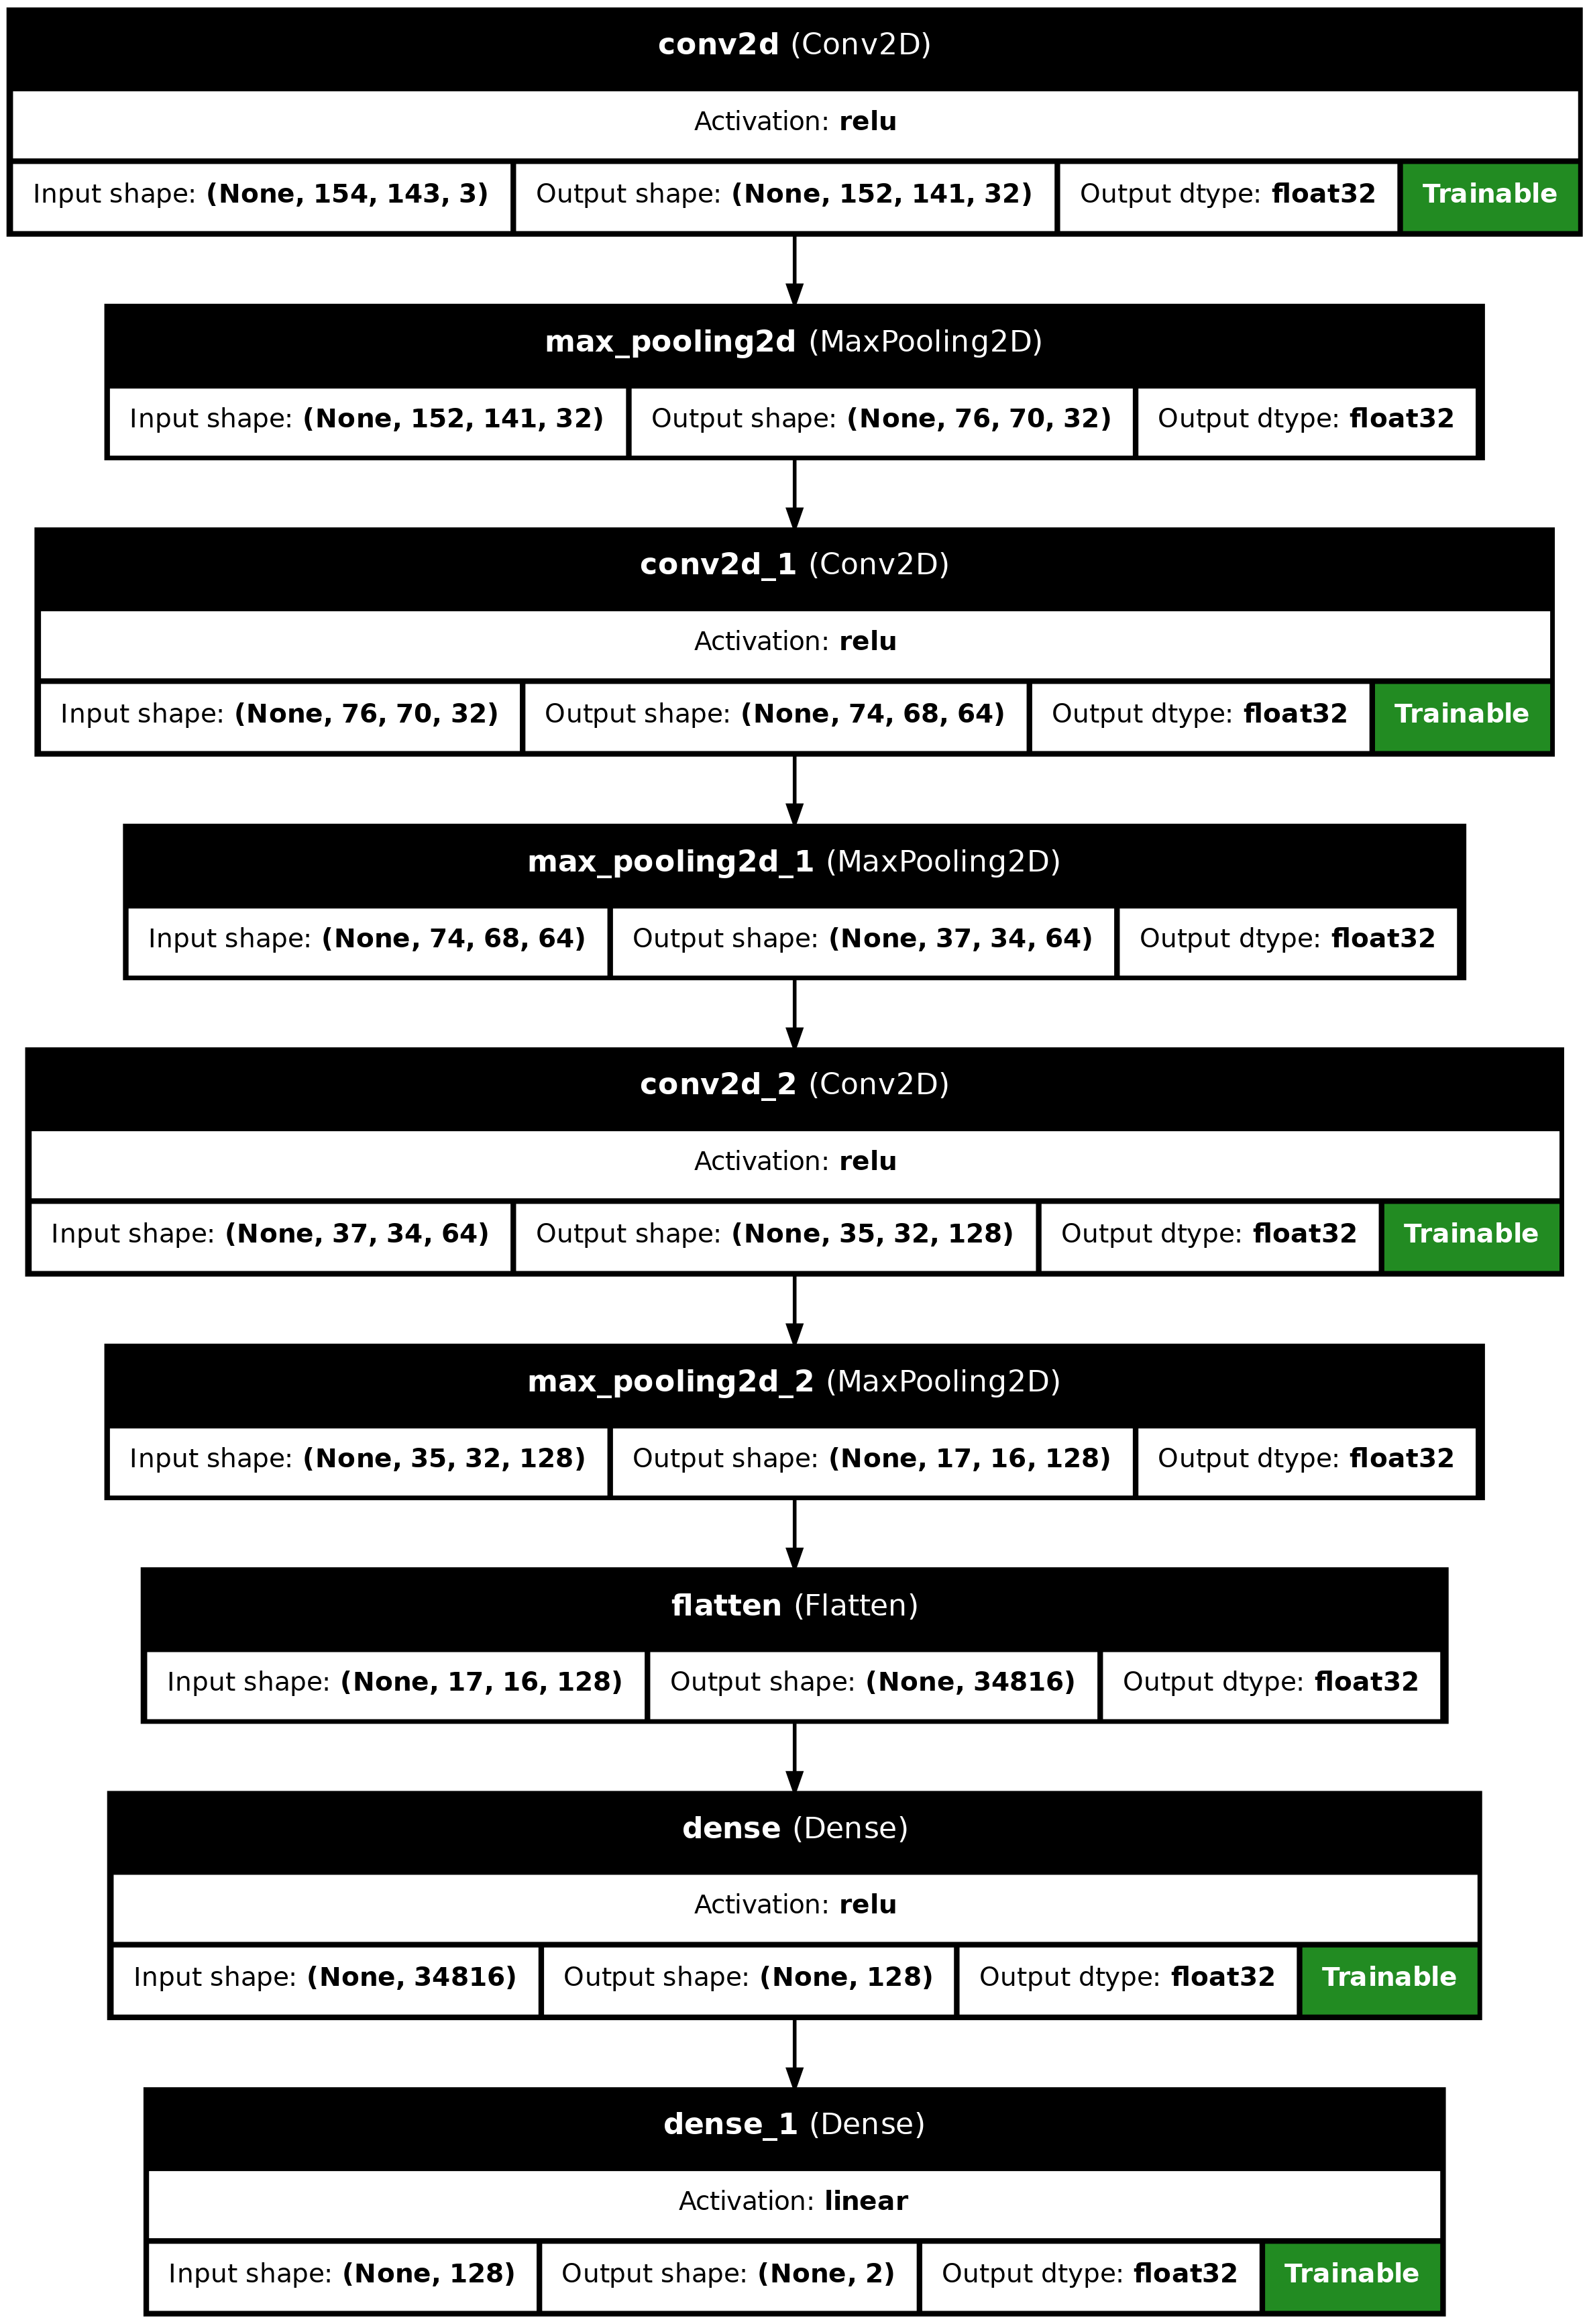
\includegraphics[width=.8\textwidth]{../photos/fiducial_coords_model}
        \caption[originalRainbow]{Fiducial coordinates model}
        \label{fig:fiducial_coords_model}
    \end{subfigure}
    \caption{Structure of the CNNs}
    \label{fig:CNN_structure}
\end{figure}
An interesting way to visualize the way the CNN works is to use gradcam to visualize the gradient of the image, which corresponds to the parts of the image the CNN is looking at.
\begin{figure}[H]
    \centering
    \includegraphics[width=0.9\textwidth]{../photos/gradcam_combined_image}
    \caption[cnn-gradcam]{Gradcam of the different layers (using another CNN which was trained to do the same task)}
    \label{fig:gradcam_combined_image}
\end{figure}

% Todo add stats about the real world training/tests
\todo{Todo add stats about the real world training/tests}


\section{Ball Detection}\label{sec:ball-detection}
The ball detection is a crucial part of the software, because if the ball is not detected correctly, the whole system will not work.
To detect ball an image is taken without the ball present and then the image with the ball is subtracted from the image without the ball, so that only the ball remains in the image.
But a problem that arises is that also other things that change are detected, like people moving or the table moving.
Luckily the glass table is so reflective and the light from the bottom is strong enough that the people behind the glass table have a low contrast in the image, so they are not detected.
To detect the ball I just filter out the white pixels in the image, because the ball is white.
The ball detection can be seen here:
\begin{figure}[H]
    \centering
    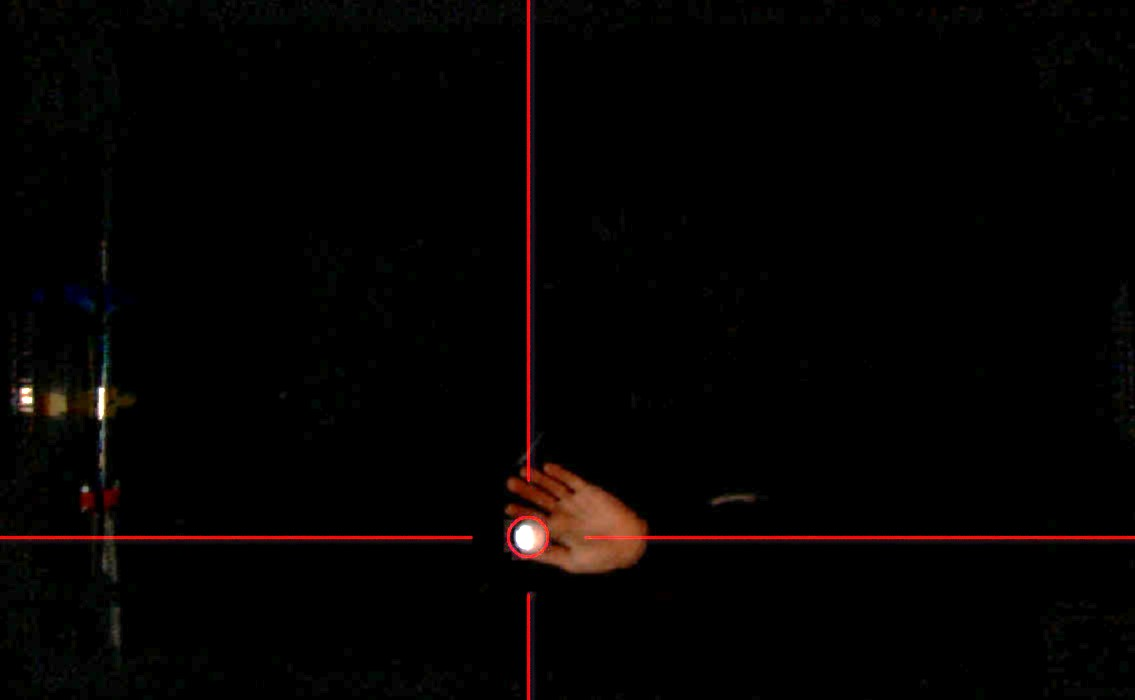
\includegraphics[width=0.9\textwidth]{../photos/ball_detection}
    \caption[ball-detection]{Ball detection in action}
    \label{fig:ball_detection}
\end{figure}
But having the pixel coordinates is not very useful, so we have to convert the pixel coordinates to real-world coordinates.
To compute the real world coordinates we compare the pixel coordinates of the ball to the pixel coordinates of the fiducials.
I measured the distance between the walls and the fiducials and made a coordinate system so that the fiducial with the number 2 lies in the top left corner (0,0) and the other fiducials are placed accordingly.
Then to compute the real world coordinates I use a homography matrix to transform the pixel coordinates to real world coordinates.
\section*{Homography Calculation}

Homography is used to map points from image coordinates to real-world coordinates.
The transformation is defined as:

\begin{equation}
    \begin{bmatrix}
        x' \\
        y' \\
        1
    \end{bmatrix}
    = H \cdot
    \begin{bmatrix}
        x \\
        y \\
        1
    \end{bmatrix}\label{eq:homography}
\end{equation}

Where:
\begin{itemize}
    \item \( (x, y) \) are the pixel coordinates,
    \item \( (x', y') \) are the real-world coordinates,
    \item \( H \) is the \( 3 \times 3 \) homography matrix.
\end{itemize}

In Python, we compute \( H \) using the $cv2.findHomography$ function:

%\begin{lstlisting}[language=python,breaklines,label={lst:python_homography}]
%homography_matrix, _ = cv2.findHomography(pixel_points, real_points)
%\end{lstlisting}

\[
    H, \text{\_} = \text{cv2.findHomography}(\text{pixel\_points}, \text{real\_points})
\]
% todo: should i explain how the homography matrix is calculated?
\todo{Should i explain how the homography matrix is calculated?}

In Rust, this matrix is applied to new pixel points via matrix multiplication and normalization.
% todo: should i explain that i save the stuff a file and then read it to save time?


\section{Prediction}\label{sec:prediction}
To predict where the ball will go in the future I use a simple linear regression model.
But first I have to check whether the ball is still flying into the same direction and with the same velocity.
This is done by using the last position and computing the current position with the current velocity.
If the difference between the prediction and the the real world position is too large then I delete the positions and start over.
\begin{figure}[H]
    \centering
    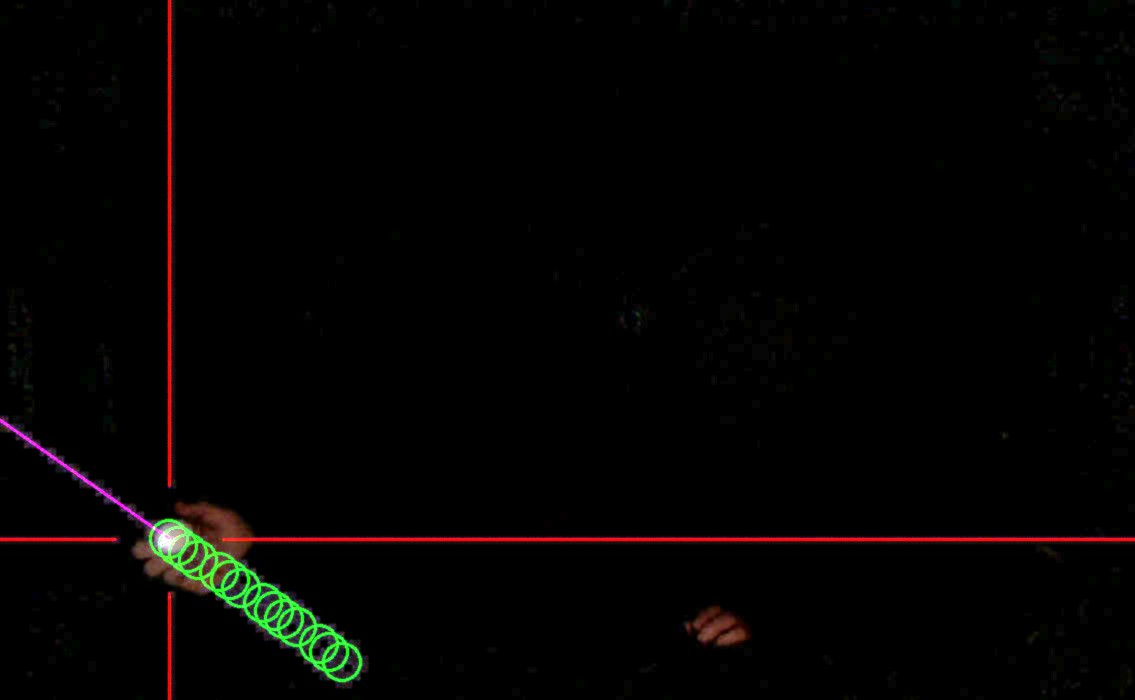
\includegraphics[width=0.9\textwidth]{../photos/ball_prediction}
    \caption[ball-prediction]{Prediction of the future positions of the ball. The green balls are the last positions and the violet line is the current velocity}
    \label{fig:ball_prediction}
\end{figure}

% todo: should i explain the linear regression model and the linear algebra behind it?
\todo{Should i explain the linear regression model and the linear algebra behind it?}
To find out where the ball will end up when it reaches the goalkepper (or any player), I can just compute the intersection between the line of the ball and the line of the goalkepper.
The line of the ball can be computed with the current position $\vec{r}$, the current velocity $\vec{v}$ and the player's $x$ coordinate.
\begin{equation}
    \begin{split}
        \vec{r} &= \begin{bmatrix}
                       x \\
                       y
        \end{bmatrix}\\
        \vec{v} &= \begin{bmatrix}
                       v_x \\
                       v_y
        \end{bmatrix}\\
%    let t = (x - self.position.x) / self.velocity.x;
%        Some(self.position + self.velocity * t)
        t &= \frac{x - r_x}{v_x}\\
        \vec{r}_\text{intersection} &= \vec{r} + \vec{v} \cdot t
    \end{split}\label{eq:ball_intersection}
\end{equation}
Now we only have to convert the $\vec{r}_\text{intersection}$ to real world coordinates and we have the position where the ball will end up, which we send to the arduino to move the stepper motor to this position.


\section{Controlling the motors}\label{sec:controlling-the-motors}
To control the motors I use an Arduino Mega 2560, because it has enough pins to control all the motors at once.
The Arduino is connected to the computer via USB, and the computer sends the motor positions to the Arduino via serial communication.

\subsubsection{Controlling the DC-Motor}\label{subsubsec:controlling-the-dc-motor}
The DC-Motor is controlled by the stepper motor driver L298N as seen here\ref{ch:electronics}.






    \chapter{Construction}\label{ch:construction}

    \section{Timeline}\label{sec:timeline}

    \chapter{Conclusion}\label{ch:conclusion}

    \section{What I learned}\label{sec:learned}

    \section{What I would do differently}\label{sec:different}

    \section{Future improvements}\label{sec:improvements}

    \section{Acknowledgements}\label{sec:acknowledgements}

    \section{References}\label{sec:references}

    \section{Appendix}\label{sec:appendix}

\end{document}

% pdflatex -interaction=nonstopmode -output-directory=output src/main.tex 
